
\documentclass[12pt]{article}

% Margen de 1 pulgada por lado
\usepackage{fullpage}
% Incluye gráficas
\usepackage{graphicx}
% Packages para matemáticas, por la American Mathematical Society
\usepackage{amssymb}
\usepackage{amsmath}
% Desactivar hyphenation
\usepackage[none]{hyphenat}
% Saltar entre párrafos - sin sangrías
\usepackage{parskip}
% Español y UTF-8
\usepackage[spanish]{babel}
\usepackage[utf8]{inputenc}
% Links en el documento
\usepackage{hyperref}
\usepackage{fancyhdr}
\setlength{\headheight}{15.2pt}
\setlength{\headsep}{5pt}
\pagestyle{fancy}

\newcommand{\N}{\mathbb{N}}
\newcommand{\Exp}[1]{\mathcal{E}_{#1}}
\newcommand{\List}[1]{\mathcal{L}_{#1}}
\newcommand{\EN}{\Exp{\N}}
\newcommand{\LN}{\List{\N}}

\newcommand{\comment}[1]{}
\newcommand{\lb}{\\~\\}
\newcommand{\eop}{_{\square}}
\newcommand{\hsig}{\hat{\sigma}}
\newcommand{\ra}{\rightarrow}
\newcommand{\lra}{\leftrightarrow}

% Cambiar por nombre completo + número de alumno
\newcommand{\alumno}{Diego Iruretagoyena - 14619164}
\newcommand{\todays}{13 de Agosto, 2018}
\rhead{Actividad 0 - \alumno}

\begin{document}
\thispagestyle{empty}
% Membrete
% PUC-ING-DCC-IIC1103
\begin{minipage}{2.3cm}

\includegraphics[width=2cm]{img/logo.pdf}
\vspace{0.5cm} % Altura de la corona del logo, así el texto queda alineado verticalmente con el círculo del logo.
\end{minipage}
\begin{minipage}{\linewidth}
\textsc{\raggedright \footnotesize
Pontificia Universidad Católica de Chile \\
Departamento de Ciencia de la Computación \\
Estructuras de Datos y Algoritmos | IIC2133 \\}
\end{minipage}


% Titul\section*{Introducion }o
\begin{center}
\vspace{0.5cm}
{\huge\bf Tarea 2}\\
\vspace{0.2cm}
\todays\\

\footnotesize{\alumno}
\rule{\textwidth}{0.05mm}
\end{center}

\section*{Introducción}

En esta oportunidad, desarrollamos 

\vspace{0.2cm}
\begin{center}
	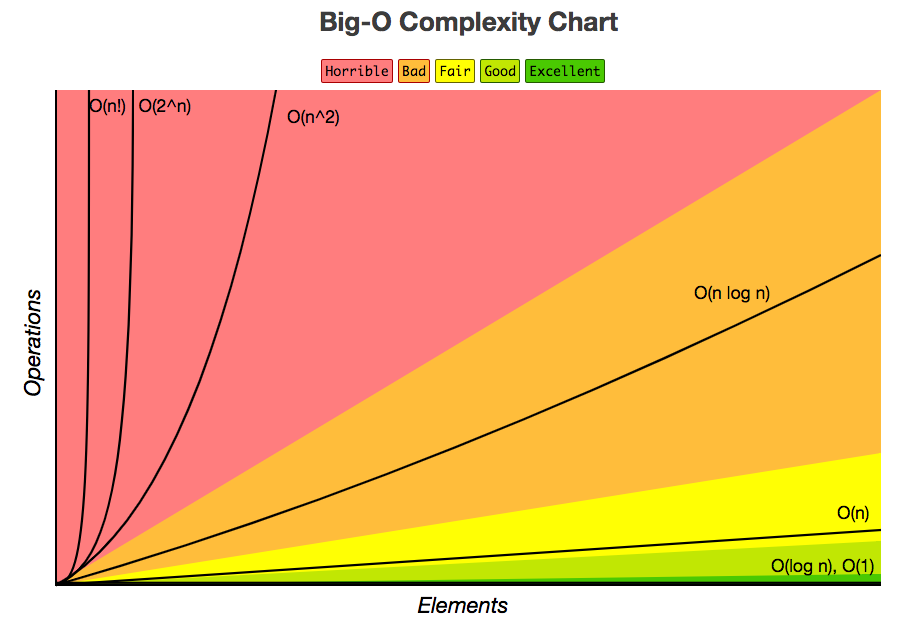
\includegraphics[width=0.5\textwidth]{img/Complex.png}
\end{center}



\section*{Análisis}


1. Análisis: 

Debes mostrar a traves de graficos la complejidad de los distintos test con respecto a su tamano. 

Especıficamente debes hacer un grafico donde el eje x corresponde a las dimensiones de la matriz (NM ) y el eje y corresponde al tiempo total que tomo tu programa en resolverlo. 

Tambien debes crear otro grafico con el mismo eje x, pero muestre en el eje y la cantidad de veces que se deshace una asignacion (cantidad de veces que se ejecuta la lınea 8 del algoritmo).


Junto con los graficos debes comentar la complejidad que crees que tiene el algoritmo viendo los datos.




\newpage
\section*{Optimizaciones}

A medida que vamos conociendo el proceso, nos damos cuenta que hay veces que el algortimo podria evitar seguir un camino, dadas ciertas condiciones. Por ejemplo, puedo evitar pensar en opciones si

analisis de este tipo nos permiten acortar los tiempos de ejecución, ya que nos hacen no gastar recursos innecesariamente en opciones que no nos serán utiles. Existen varias formas de realizar estos ajustes al comportamiento de nuestro programa, siendo las principales las \textbf{podas}, las \textbf{heuristicas} y las \textbf{propagaciones}.
A continuación explicaremos que es cada una de esas, pra luego dar ejemplos concretos de como podemos aplicarlo a nuestro problema.


explicando brevemente la forma de implementarlo y por que se espera que esto mejore la eficiencia del algoritmo.





\textbf{1. Poda}

Podas: una poda busca descartar combinaciones que no llegar´an a resolver el problema independiente
de que no est´en incumpliendo alguna restricci´on actualmente, por lo que una poda para hacer m´as eficiente
el algoritmo es que si se est´a cumpliendo una restricci´on de una fila todos los espacios de imanes horizontales
restantes que est´an en esa fila ser´an vac´ıos y si se est´a cumpliendo una restricci´on de una columna todos
los espacios de imanes verticales restantes que est´an en esa columna ser´an vac´ıos. En los dos casos permite
ahorrar tiempo en revisar todas esas celdas que de antemano se sabe que no se puede poner nada ya que
no se seguir´a cumpliendo con la restricci´on correspondiente. Por ejemplo, se est´a haciendo el test 6 y se ha
hecho la primera asignaci´on, quedando de la siguiente manera:


Se puede ver que en la segunda columna ya se cumpli´o con la restricci´on de positivos, por lo que si se
asigna cualquier im´an vertical se dejar´a de cumplir con esta restricci´on. Esto permite ahorrarse revisar tres
espacios verticales de inmediato. Si esto se hace durante todo el proceso permitir´ıa evitarse buscar en una
gran cantidad de cambinaciones, lo que lleva a una gran reducci´on en el tiempo que demora el proceso.



\textbf{2. Heurística}

Heur´ıstica: para desarrollar el problema de manera m´as efectiva, se puede cambiar el orden en que se
va armando el tablero. En lugar de empezar recorriendo cada fila y cada columna dentro de esta (o al rev´es),
se le puede dar una prioridad a cada celda y de acuerdo a esto ir armando el tablero. Una buena manera
de establecer prioridades es de acuerdo a lo acotado que est´a su dominio, lo que se puede establecer por
medio de las restricciones que tiene. Para realizar esto se pueden sumar las restricciones que hay para cada
celda, es decir, filas positivas y negativas y columnas positivas y negativas. Para esto no importa el signo de
la restricci´on, ya que la heur´ıstica solo busca que primero se vean celdas que probablemente no terminar´an
vac´ıas. Por ejemplo, en el test 4 la soluci´on es de la siguiente forma:



\textbf{3. Propagacion}
y una manera de propagar en este problema 


Al ir viendo las prioridades, se tiene que la celda (0,0) tiene prioridad 6, la celda (1,0) tambi´en (fila +3 y
columna -3) y la (2,0) tiene prioridad 4. Luego de que se le da una prioridad a cada celda, se realiza el mismo
procedimiento de antes pero se revisan las celdas con mayor prioridad primero, hasta llegar a las que tengan
prioridad 0. Esta heur´ıstica permite evitar de cierta manera poner celdas que con mayor probabilidad se
tengan que sacar despu´es ya que la soluci´on es con ese espacio vac´ıo y que no se tenga que volver hasta la
ra´ız al hacer el backtracking.
Propagaci´on: una propagaci´on bastante simple si se realiza el c´odigo revisando por celdas es que si se
pone una celda positiva, la celda que acompa˜na en el espacio que comparten debe ser negativa y si se pone
una negativa la que la acompa˜na en el espacio que comparten debe ser positiva. Esta propagaci´on es bastante
obvia, ya que ser´ıa sumamente ineficiente no hacerlo de esta manera ya que se revisar´ıa una celda que de
antemano se sabr´ıa el valor que tiene que tener para cumplir con la restricci´on de que dos celdas aleda˜nas
deben tener carga contraria en caso de no estar vac´ıas.









% Fin del documento
\end{document}
